\def\documentauthor{Carlos Salinas}
\def\documenttitle{MA571 Homework \hwnum}
\def\hwnum{9}
\def\shorttitle{MA571 HW \hwnum}
\def\coursename{MA571}
\def\documentsubject{point-set topology}
\def\authoremail{salinac@purdue.edu}

\documentclass[article,oneside,10pt]{memoir}
\usepackage{geometry}
\usepackage[dvipsnames]{xcolor}
\usepackage[
    breaklinks,
    bookmarks=true,
    colorlinks=true,
    pageanchor=false,
    linkcolor=black,
    anchorcolor=black,
    citecolor=black,
    filecolor=black,
    menucolor=black,
    runcolor=black,
    urlcolor=black,
    hyperindex=false,
    hyperfootnotes=true,
    pdftitle={\shorttitle},
    pdfauthor={\documentauthor},
    pdfkeywords={\documentsubject},
    pdfsubject={\coursename}
    ]{hyperref}

% Use symbols instead of numbers
\renewcommand*{\thefootnote}{\fnsymbol{footnote}}

\usepackage{graphicx}
\graphicspath{{figures/}}

% Misc
\usepackage{microtype}
\usepackage{multicol}
\usepackage[inline]{enumitem}
\usepackage{listings}
\usepackage{mleftright}
\mleftright

%% Math
\usepackage{amsthm}
\usepackage{amssymb}
\usepackage{mathtools}
% \usepackage{unicode-math}

%% PDFTeX specific
\usepackage[mathcal]{euscript}
\usepackage{mathrsfs}

\usepackage{cmap}
\usepackage[T2A,T1]{fontenc}
\usepackage[utf8]{inputenc}
\usepackage[french,german,russian,spanish,english]{babel}
\babeltags{fr=french,
           de=german,
           ru=russian,
           es=spanish,
           en=english}
\def\spanishoptions{mexico}
\usepackage{CJKutf8}
\newcommand{\textha}[1]{\begin{CJK}{UTF8}{mj}#1\end{CJK}}
\newcommand{\textni}[1]{\begin{CJK}{UTF8}{min}#1\end{CJK}}
\newcommand{\textzh}[1]{\begin{CJK}{UTF8}{bsmi}#1\end{CJK}}

%% Theorems and definitions
\theoremstyle{plain}
\newtheorem{theorem}{Theorem}
\newtheorem{proposition}[theorem]{Proposition}
\newtheorem{corollary}[theorem]{Corollary}
\newtheorem{claim}[theorem]{Claim}
\newtheorem{lemma}[theorem]{Lemma}
\newtheorem{axiom}[theorem]{Axiom}

\newtheorem*{corollary*}{Corollary}
\newtheorem*{claim*}{Claim}
\newtheorem*{lemma*}{Lemma}
\newtheorem*{proposition*}{Proposition}
\newtheorem*{theorem*}{Theorem}

\theoremstyle{definition}
\newtheorem{definition}{Definition}
\newtheorem{example}{Examples}
\newtheorem{examples}[example]{Examples}
% \newtheorem{exercise}{Exercise}[section]
% \newtheorem{problem}[exercise]{Problem}

% \newtheorem{exercise}{Exercise}[section]
% \newtheorem{problem}[exercise]{Problem}

\newcounter{problem}
\newenvironment{problem}[1][]% environment name
{% begin code
  \stepcounter{problem}
  \par\vspace{\baselineskip}\noindent
  \ifx &#1&%
  {\normalfont\Large\bfseries\scshape Problem~\hwnum.\theproblem}
  \global\def\exercisename{Problem~\hwnum.\theproblem}%
  \else
  {\normalfont\Large\bfseries\scshape Problem~\hwnum.\theproblem~(#1)}
  \global\def\exercisename{Problem~\hwnum.\theproblem(#1)}
  \fi
  \par\vspace{\baselineskip}%
  \noindent\ignorespaces
}%
{% end code
  \par\vspace{\baselineskip}%
  \noindent\ignorespacesafterend
}

\newtheorem*{definition*}{Definition}
\newtheorem*{example*}{Examples}
\newtheorem*{examples*}{Examples}
\newtheorem*{exercise*}{Exercise}
\newtheorem*{problem*}{Problem}

\theoremstyle{remark}
\newtheorem{remark}{Remark}
\newtheorem{remarks}[remark]{Remarks}
\newtheorem{observation}[remark]{Observation}
\newtheorem{observations}[remark]{Observations}

\newtheorem*{remark*}{**Remark**}
\newtheorem*{remarks*}{**Remarks**}
\newtheorem*{observation*}{**Observation**}
\newtheorem*{observations*}{**Observations**}

%% Redefinitions & commands
\newcommand\restr[2]{{% we make the whole thing an ordinary symbol
  \left.\kern-\nulldelimiterspace % automatically resize the bar with \right
  {#1} % the function
  % \vphantom{\big|} % pretend it's a little taller at normal size
  \right|{#2} % this is the delimiter
  }}

\newcommand{\nsubset}{\ensuremath{\not\subset}}
\newcommand{\nsupset}{\ensuremath{\not\supset}}
\renewcommand\qedsymbol{\ensuremath{\null\hfill\blacksquare}}

%% Commands and operators
\DeclareMathOperator{\diam}{diam}
\DeclareMathOperator{\id}{id}
\DeclareMathOperator{\im}{im}
\DeclareMathOperator{\Int}{int}
\DeclareMathOperator{\Cl}{cl}

\newcommand{\CC}{\mathbb{C}}
\newcommand{\NN}{\mathbb{N}}
\newcommand{\QQ}{\mathbb{Q}}
\newcommand{\RR}{\mathbb{R}}
\newcommand{\ZZ}{\mathbb{Z}}

% Renewcommands
% \renewcommand\setminus{\smallsetminus}
\renewcommand\phi{\varphi}
\renewcommand\epsilon{\varepsilon}

\begin{document}
\frontmatter
\aliaspagestyle{title}{empty}
\pagestyle{title}
\author{\href{mailto:\authoremail}{\documentauthor}}
\title{\documenttitle}
\date{\today}
\maketitle
\cleartooddpage

\makeoddhead{headings}
        {\small{\MakeUppercase{\itshape\documentauthor}}}
        {}
        {\small{\MakeUppercase{\itshape\exercisename}}}
\makeoddfoot{headings}{{\itshape\documenttitle}}
                      {}
                      {\thepage}
\makeevenhead{headings}
        {\small{\MakeUppercase{\itshape\documentauthor}}}
        {}
        {\small{\MakeUppercase{\itshape\exercisename}}}
\makeevenfoot{headings}{{\itshape\documenttitle}}
                      {}
                      {\thepage}
\makeheadrule{headings}{\textwidth}{.25pt}
% \makerunningwidth{headings}{1.15\textwidth}
\pagestyle{headings}

\mainmatter
% \setcounter{theorem}{16}
\begin{problem}[Munkres \S52, Ex.\,2]
Let $\alpha$ be a path in $X$ from $x_0$ to $x_1$; let $\beta$ be
a path in $X$ from $x_1$ to $x_2$. Show that if
$\gamma=\alpha*\beta$, then $\hat\gamma=\hat\beta\circ\hat\alpha$.
\end{problem}
\begin{proof}
By Theorem 52.1, the paths $\alpha$ and $\beta$ induce a group homomorphism
$\hat\alpha\colon\pi_1(X,x_0)\to\pi_1(X,x_1)$ and
$\hat\beta\colon\pi_1(X,x_1)\to\pi_1(X,x_2)$, respectively. We want to
show therefore that the induced homomorphism
$\hat\gamma=\widehat{\alpha*\beta}$ is in fact equivalent to the
composition $\hat\beta\circ\hat\alpha$. Let $[f]$ be a loop based at $x_0$
then
\begin{align*}
\hat\gamma([f])&=\widehat{\alpha*\beta}([f])\\
               &=\bigl[\,\overline{\alpha*\beta}\,\bigr]*[f]*[\alpha*\beta]\\
               &=\bigl[\bar\beta*\bar\alpha\bigr]*[f]*[\alpha]*[\beta]\\
\shortintertext{by the well-definedness of the path product operation, we have}
               &=[\bar\beta]*[\bar\alpha]*[f]*[\alpha]*[\beta]\\
\shortintertext{by associativity of the path product,}
               &=[\bar\beta]*([\bar\alpha]*[f]*[\alpha])*[\beta]\\
               &=[\bar\beta]*\hat\alpha([f])*[\beta]\\
\shortintertext{where $\alpha([f])$ is a loop based at $x_1$ so}
               &=\hat\beta\left(\hat\alpha([f])\right)\\
               &=\bigl(\hat\beta\circ\hat\alpha\bigr)([f]).
\end{align*}
Thus, the following diagram commutes
\begin{center}
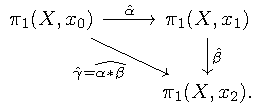
\includegraphics{figures/hw-10-pi-1-path-diagram}
\end{center}
\end{proof}
\newpage
\begin{problem}[Munkres \S52, Ex.\,3]
Let $x_0$ and $x_1$ be points of the path-connected space
$X$. Show that $\pi_1(X,x_0)$ is Abelian if and only if for every
pair $\alpha$ and $\beta$ of paths from $x_0$ to $x_1$, we have
$\hat\alpha=\hat\beta$.
\end{problem}
\begin{proof}
$\implies$ Suppose that $\pi_1(X,x_0)$ is Abelian. Then for any class of
loops about $x_0$, say $[f]$ and $[g]$, the product $[f]*[g]=[g]*[f]$. Let
$\alpha$ and $\beta$ be paths from $x_0$ to $x_1$. Then the induced map on
fundamental groups $\hat\alpha$ and $\hat\beta$ yield isomorphism by
Theorem 52.1 so that the map $\hat{\bar\beta}\circ\hat\alpha$ is an
automorphism of $\pi_1(X,x_0)$. Moreover, we have
\begin{align*}
\hat{\bar{\beta}}\circ\hat\alpha([f])
&=
\hat{\bar{\beta}}\bigl(\hat\alpha([f])\bigr)\\
&=
\hat{\bar{\beta}}\bigl([\bar\alpha]*[f]*[\alpha]\bigr)\\
&=
[\beta]*\bigl([\bar\alpha]*[f]*[\alpha]\bigr)*[\bar\beta]\\
\shortintertext{by associativity of the path product, we may rewrite the
  above expression as}
&=([\beta]*[\bar\alpha])*[f]*([\alpha]*[\bar\beta])
\shortintertext{noting that $[\beta]*[\bar\alpha]$ and
  $[\alpha]*[\bar\beta]$ are loops based at $x_0$, since $\pi_1(X,x_0)$ is
  Abelian, we have}
&=([\beta]*[\bar\alpha])*([\alpha]*[\bar\beta])*[f]\\
&=[e_{x_0}]*[f]\\
&=[f].
\end{align*}
Thus, $\hat{\bar{\beta}}\circ\hat\alpha=\id_{\pi_1(X,x_0)}$, i.e.,
$\hat\alpha=\hat\beta$.

$\impliedby$ Let $f$ and $g$ be loops about $x_0$. Then, since $X$ is path
connected, we claim that $f$ and $g$ are homotopic to the path product
$\alpha_1*\bar\beta_1$ and $\alpha_2*\bar\beta_2$ where $\alpha_i,\beta_i$
are paths from $x_0$ to $x_1$. More precisely, split $f$ into the paths
$f_1=f(t/2)$ and $f_2=f((t+1)/2)$; it is clear that $f=f_1*f_2$. Let
$x_2\coloneqq f_1(1)$ then there exists a path $\alpha$ from $x_2$ to $x_1$
since $X$ is path connected. Now we claim that the following
\[
H(x,t)\coloneqq f_1(x)*\alpha(tx)*\bar\alpha((1-t)x)*f_2(x)
\]
is a homotopy from $f=f_1*f_2$ to the extended loop $\tilde
f=f_1*\alpha*\bar\alpha*f_2$.
\begin{proof}[Proof of claim]
\renewcommand{\qedsymbol}{$\clubsuit$}
It is clear that $H$ is continuous since it is
a path products and multiplication on the unit interval $I$ is
continuous so $tx$ is continuous. Lastly,
$H(x,0)=f_1(x)*\alpha(0)*\bar\alpha(0)*f_2(x)$ and
$H(x,1)=f_1(x)*\alpha(x)*\bar\alpha(x)*f_2(x)$.
\end{proof}
Now, let $f\simeq_p\alpha_1*\bar\beta_1$ and
$g\simeq_p\alpha_2*\bar\beta_2$ where $\alpha_i,\beta_i$ are
paths from $x_0$ to $x_1$. Then we have
\begingroup
\allowdisplaybreaks
\begin{align*}
[f]*[g]*[\bar f]*[\bar g]
&=
[\alpha_1*\bar\beta_1]*[\alpha_2*\bar\beta_2]*
\bigl[\overline{\alpha_1*\bar\beta_1}\bigr]*
\bigl[\overline{\alpha_2*\bar\beta_2}\bigr]\\
&=
[\alpha_1*\bar\beta_1]*[\alpha_2*\bar\beta_2]*
[\beta_1*\bar\alpha_1]*[\beta_2*\bar\alpha_2]\\
&=
[\alpha_1]*[\bar\beta_1]*[\alpha_2]*[\bar\beta_2]*
[\beta_1]*[\bar\alpha_1]*[\beta_2]*[\bar\alpha_2]\\
&=\hat{\bar{\alpha}}_1\bigl([\bar\beta_1]*[\alpha_2]*[\bar\beta_2]*[\beta_1]\bigr)*[\beta_2]*[\alpha_2]\\
&=\hat{\bar{\alpha}}_1\bigl(\hat\beta_2([\alpha_2]*[\bar\beta_2])\bigr)*[\beta_2]*[\bar\alpha_2]\\
&=[\alpha_2]*[\bar\beta_2]*[\beta_2]*[\bar\alpha_2]\\
&=[\alpha_2]*[e_{x_0}]*[\bar\alpha_2]\\
&=[\alpha_2]*[\bar\alpha_2]\\
&=[e_{x_0}].
\end{align*}
\endgroup
Thus, $\pi_1(X,x_0)$ is Abelian.
\end{proof}
\newpage
\begin{problem}[Munkres \S52, Ex.\,4]
Let $A\subset X$; suppose $r\colon X\to A$ is continuous map such
that $r(a)=a$ for each $a\in A$. (The map $r$ is called a
\emph{retraction} of $X$ onto $A$.) If $a_0\in A$, show that
\[
r_*\colon\pi_1(X,x_0)\longrightarrow\pi_1(A,a_0)
\]
is surjective.
\end{problem}
\begin{proof}
\end{proof}
\newpage
\begin{problem}[Munkres \S53, Ex.\,6]
Show that if $X$ is path connected, the homomorphism induced by a
continuous map is independent of the base point, up to
isomorphisms of the groups involved. More precisely, let $h\colon
X\to Y$ be continuous, with $h(x_0)=y_0$ and $h(x_1)=y_1$. Let
$\alpha$ be a path in $X$ from $x_0$ to $x_1$, and let
$\beta=h\circ\alpha$. Show that
\[
\hat\beta\circ(h_{x_0})_*=(h_{x_1})\circ\hat\alpha.
\]
This equation expresses the fact that the following diagram of
maps ``commutes''
\begin{center}
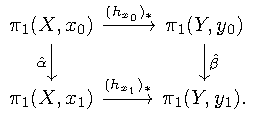
\includegraphics{figures/hw-10-path-connected-hom-indep}
\end{center}
\end{problem}
\begin{proof}
\end{proof}
\newpage
\begin{problem}[Munkres \S55, Ex.\,1]
Show that if $A$ is a retract of $B^2$, then every continuous map
$f\colon A\to A$ has a fixed point.
\end{problem}
\begin{proof}
\end{proof}
\newpage
\begin{problem}[Munkres \S55, Ex.\,2]
Show that if $h\colon S^1\to S^1$ is nulhomotopic, then $h$ has a
fixed point and $h$ maps some point $x$ to its antipode $-x$.
\end{problem}
\begin{proof}
\end{proof}
\newpage
\begin{problem}[(A)]
Prove that every $m$-manifold is locally path-connected.
\end{problem}
\begin{proof}
\end{proof}
\newpage
\begin{problem}[(B)]
Prove that every $m$-manifold is regular.
\end{problem}
\begin{proof}
\end{proof}
\newpage
\begin{problem}[(C)]
Prove that there is no $1$-$1$ continuous function $\iota\colon
S^1\to\RR$. You may assume any fact about trigonometric
functions. (Note: this shows in particular that there is no
$\iota\colon S^1\to\RR$ with $p\circ\iota$ equal to the identity
map, where $p$ is the map in the note on the Fundamental Group of
the Circle.)
\end{problem}
\begin{proof}
\end{proof}
\newpage
\begin{problem}[(D)]
Prove Proposition C from the note on the Fundamental Group of the Circle.
\end{problem}
\begin{proof}
\end{proof}

%%% Local Variables:
%%% mode: latex
%%% TeX-master: "../MA571-HW-Current"
%%% End:

\end{document}

%%% Local Variables:
%%% mode: latex
%%% TeX-master: t
%%% End:
